\chapter{System Models}
\label{ch:models}

\section{Use case diagram}
Figure~\ref{fig:usecase} shows four actors and fourteen use cases. Three actors are people; the risk engine is a system actor. Submitting work always includes a risk score. Holding the payment on-chain extends the scoring use case and happens only when the score is 0.65 or higher. The arbiter can release or refund a held payment but cannot send the money anywhere else.

\begin{sidewaysfigure}
\centering
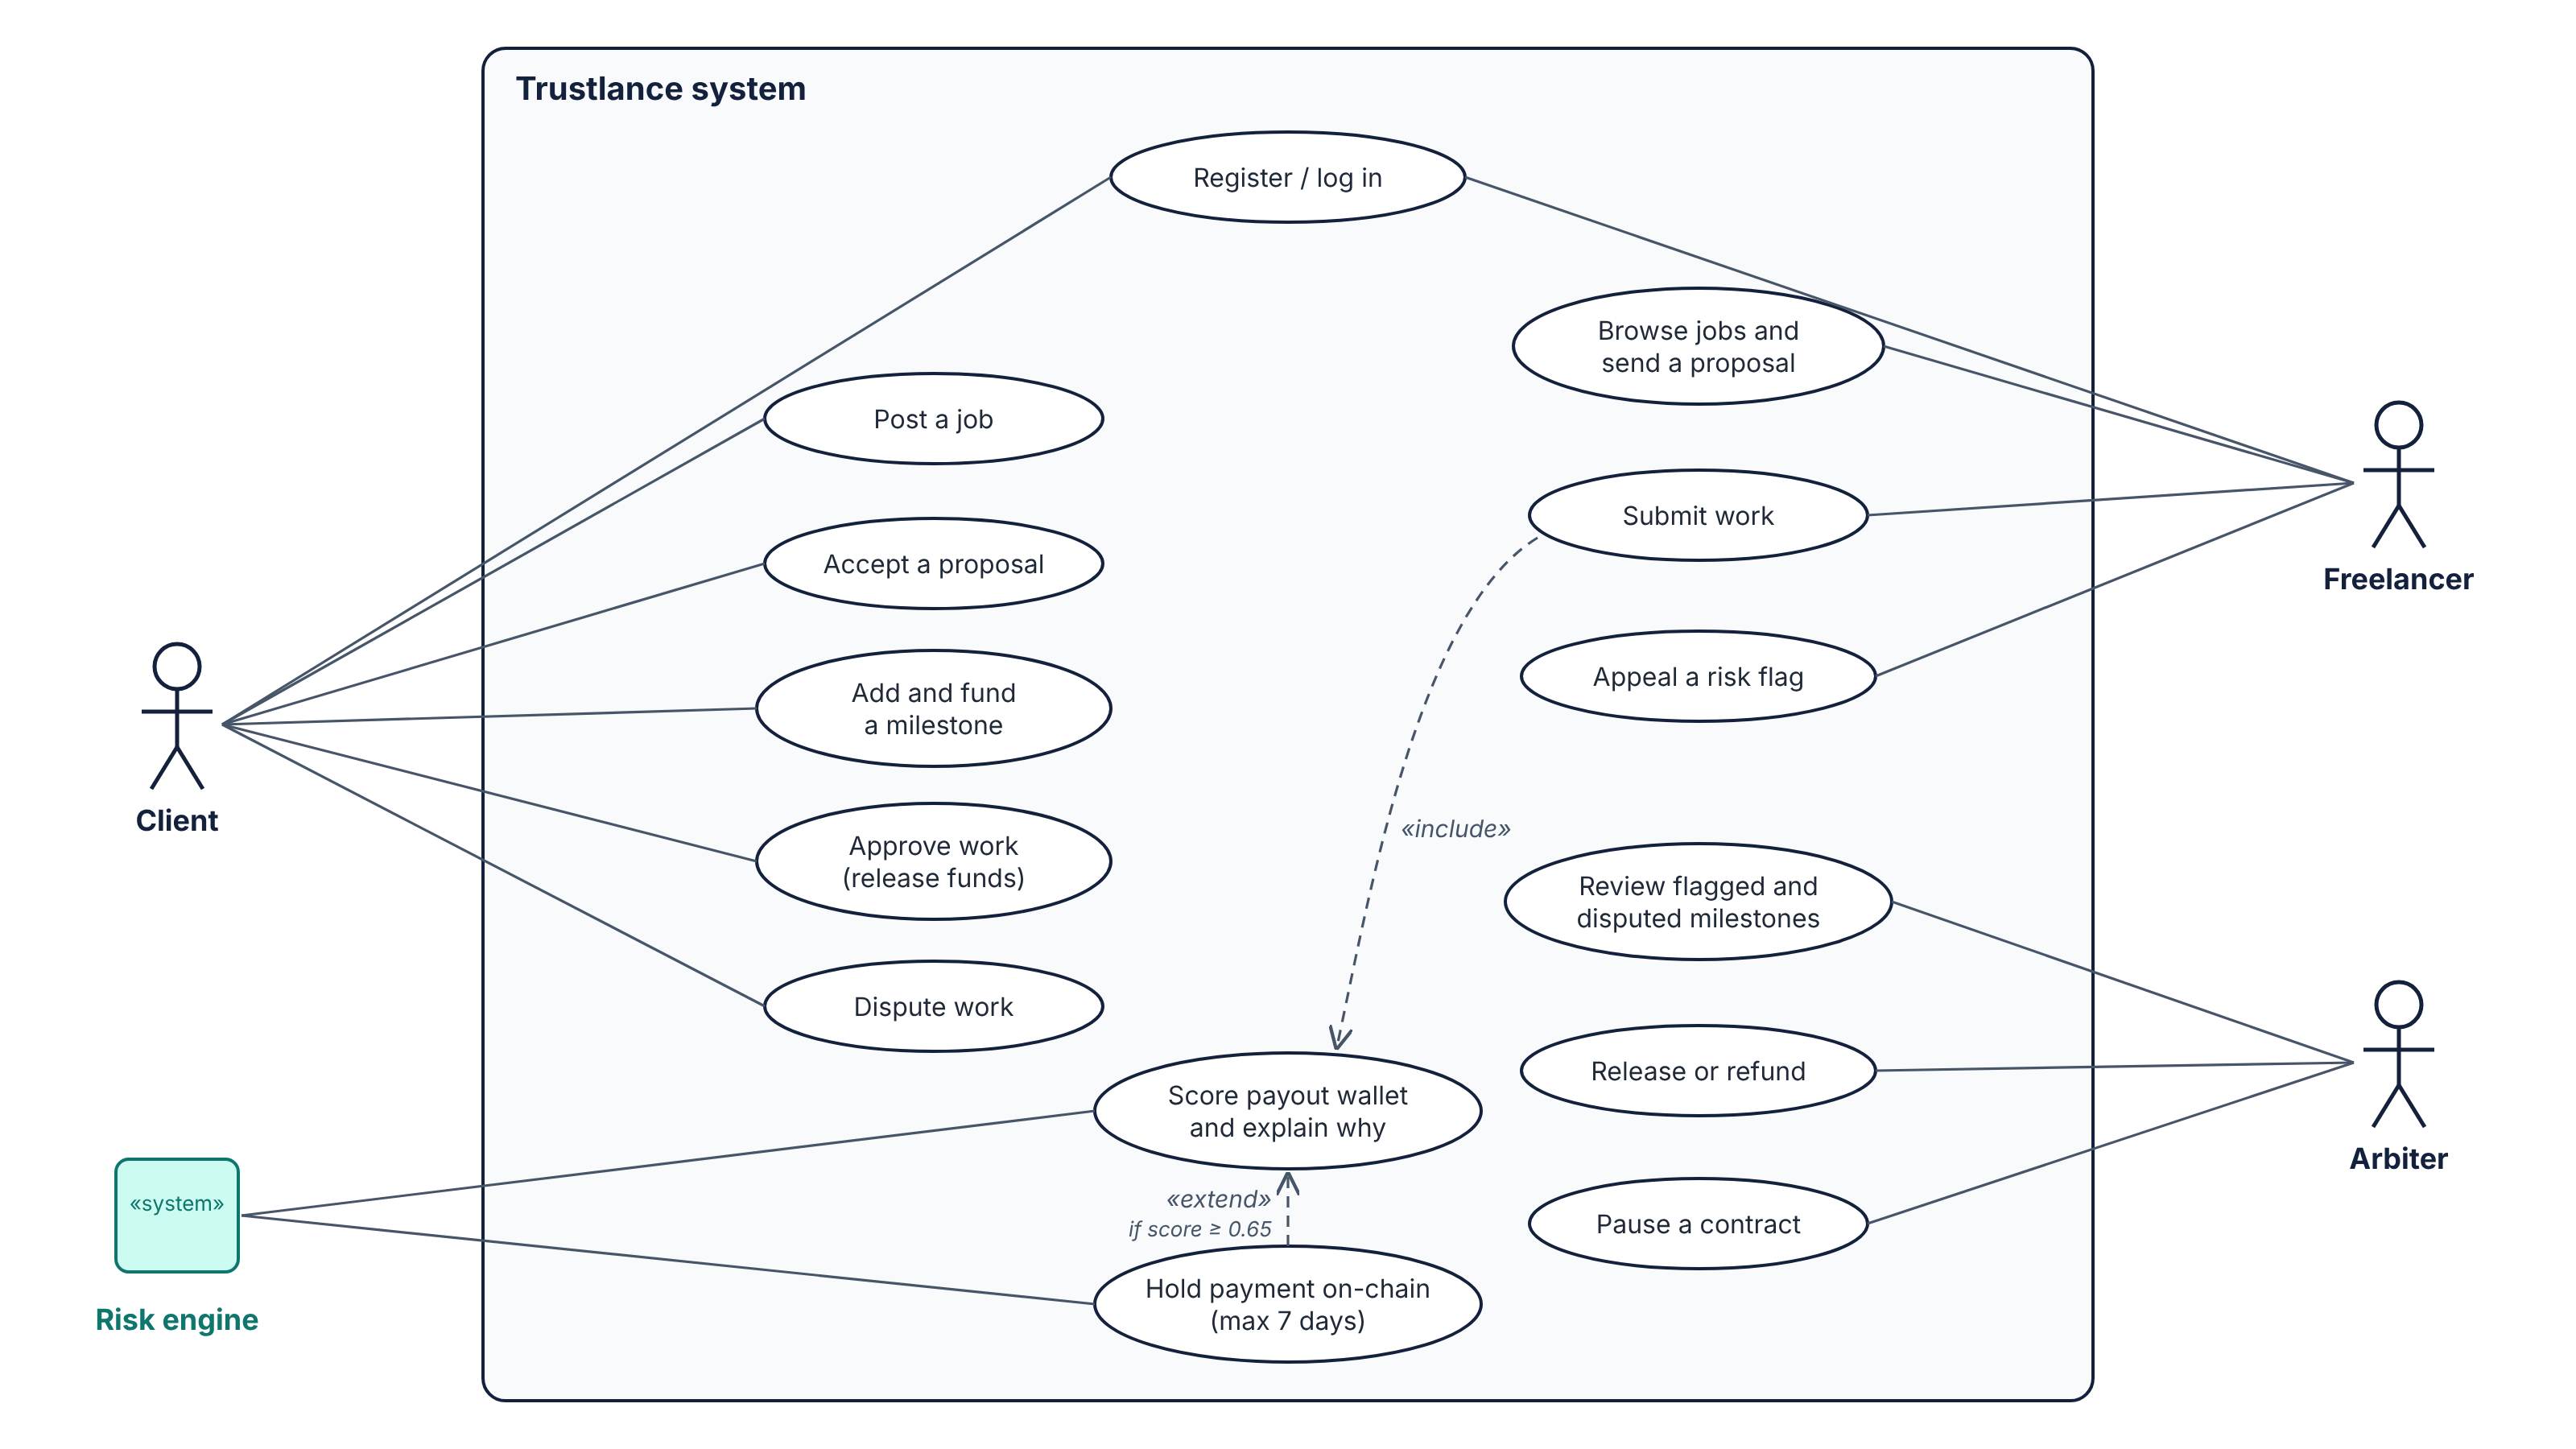
\includegraphics[width=0.95\textheight]{figures/usecase.png}
\caption{Use case diagram.}
\label{fig:usecase}
\end{sidewaysfigure}

\section{Activity diagram}
Figure~\ref{fig:activity} follows one milestone payment across four swimlanes. The client accepts a proposal, which deploys the escrow contract, and funds the milestone. The freelancer submits work and the risk engine scores the payout wallet. A low or medium score sends the milestone straight to the client, whose approval releases the funds. A high score puts the flag and its reason on-chain. From then on the client's approval is refused, the freelancer may appeal, and the arbiter decides whether to release or refund. If the arbiter does nothing for seven days, the client's approval works again. The client can also dispute submitted work at any time, which sends it to the arbiter.

\begin{sidewaysfigure}
\centering
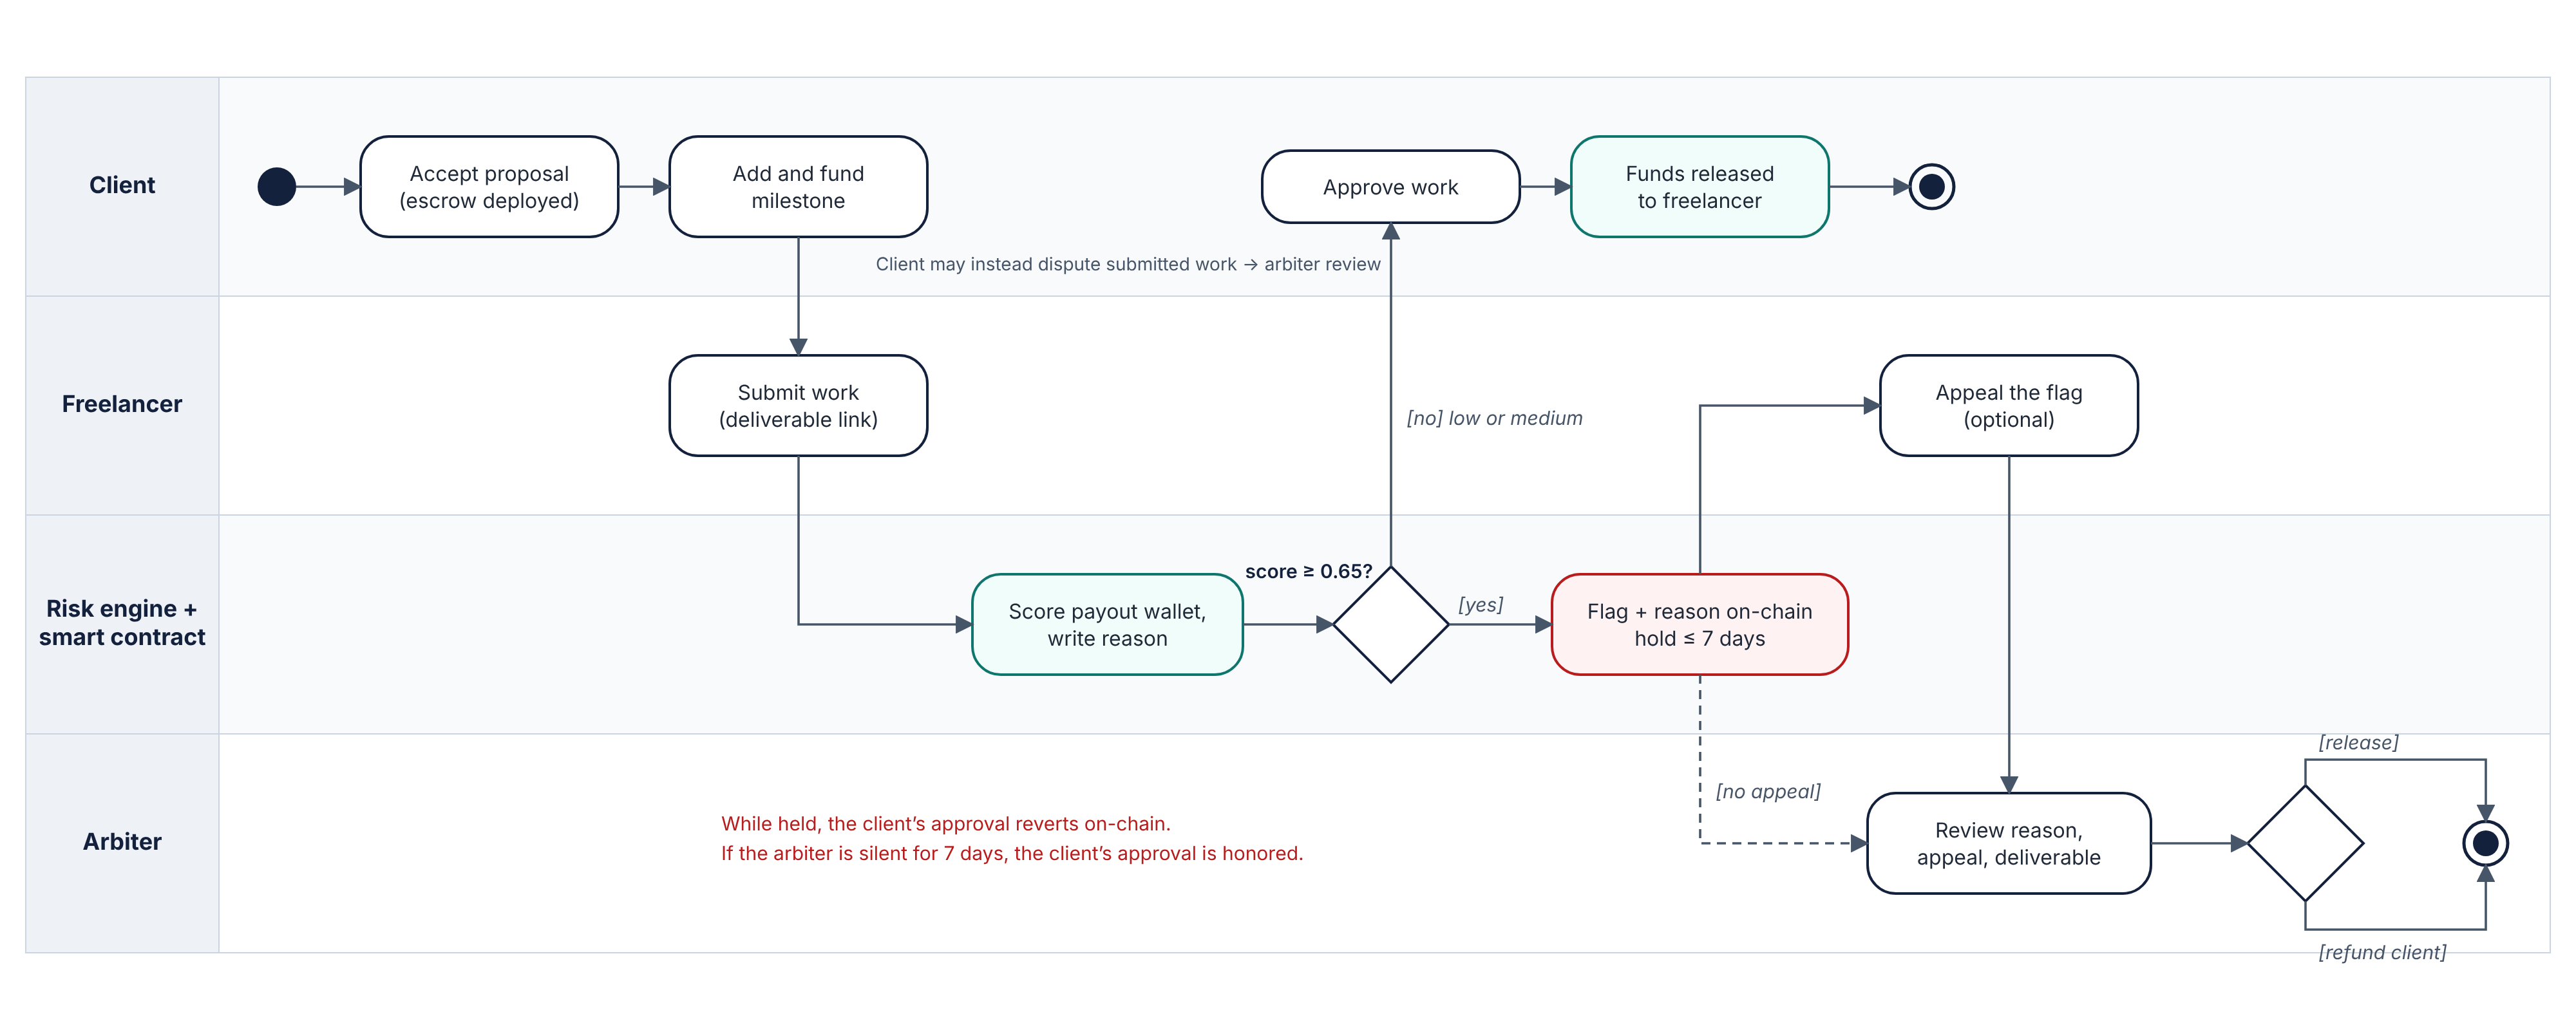
\includegraphics[width=\textheight]{figures/activity.png}
\caption{Activity diagram for one milestone payment.}
\label{fig:activity}
\end{sidewaysfigure}

\section{Entity-relationship diagram}
The database has eight tables (Figure~\ref{fig:er}). Users, jobs and milestones are the core. A job stores the address of its escrow contract and a milestone stores its index inside that contract, so the API can always read the milestone back from the chain. \texttt{risk\_assessments} keeps every score with its band, action and reason, plus the hash that links it to the tamper-evident log. \texttt{milestone\_events} records who did what and the transaction hash. \texttt{reviews} and \texttt{notifications} already exist for FR16 and FR17. The full schema is in \texttt{server/db/schema.sql}.

\begin{figure}[htbp]
\centering
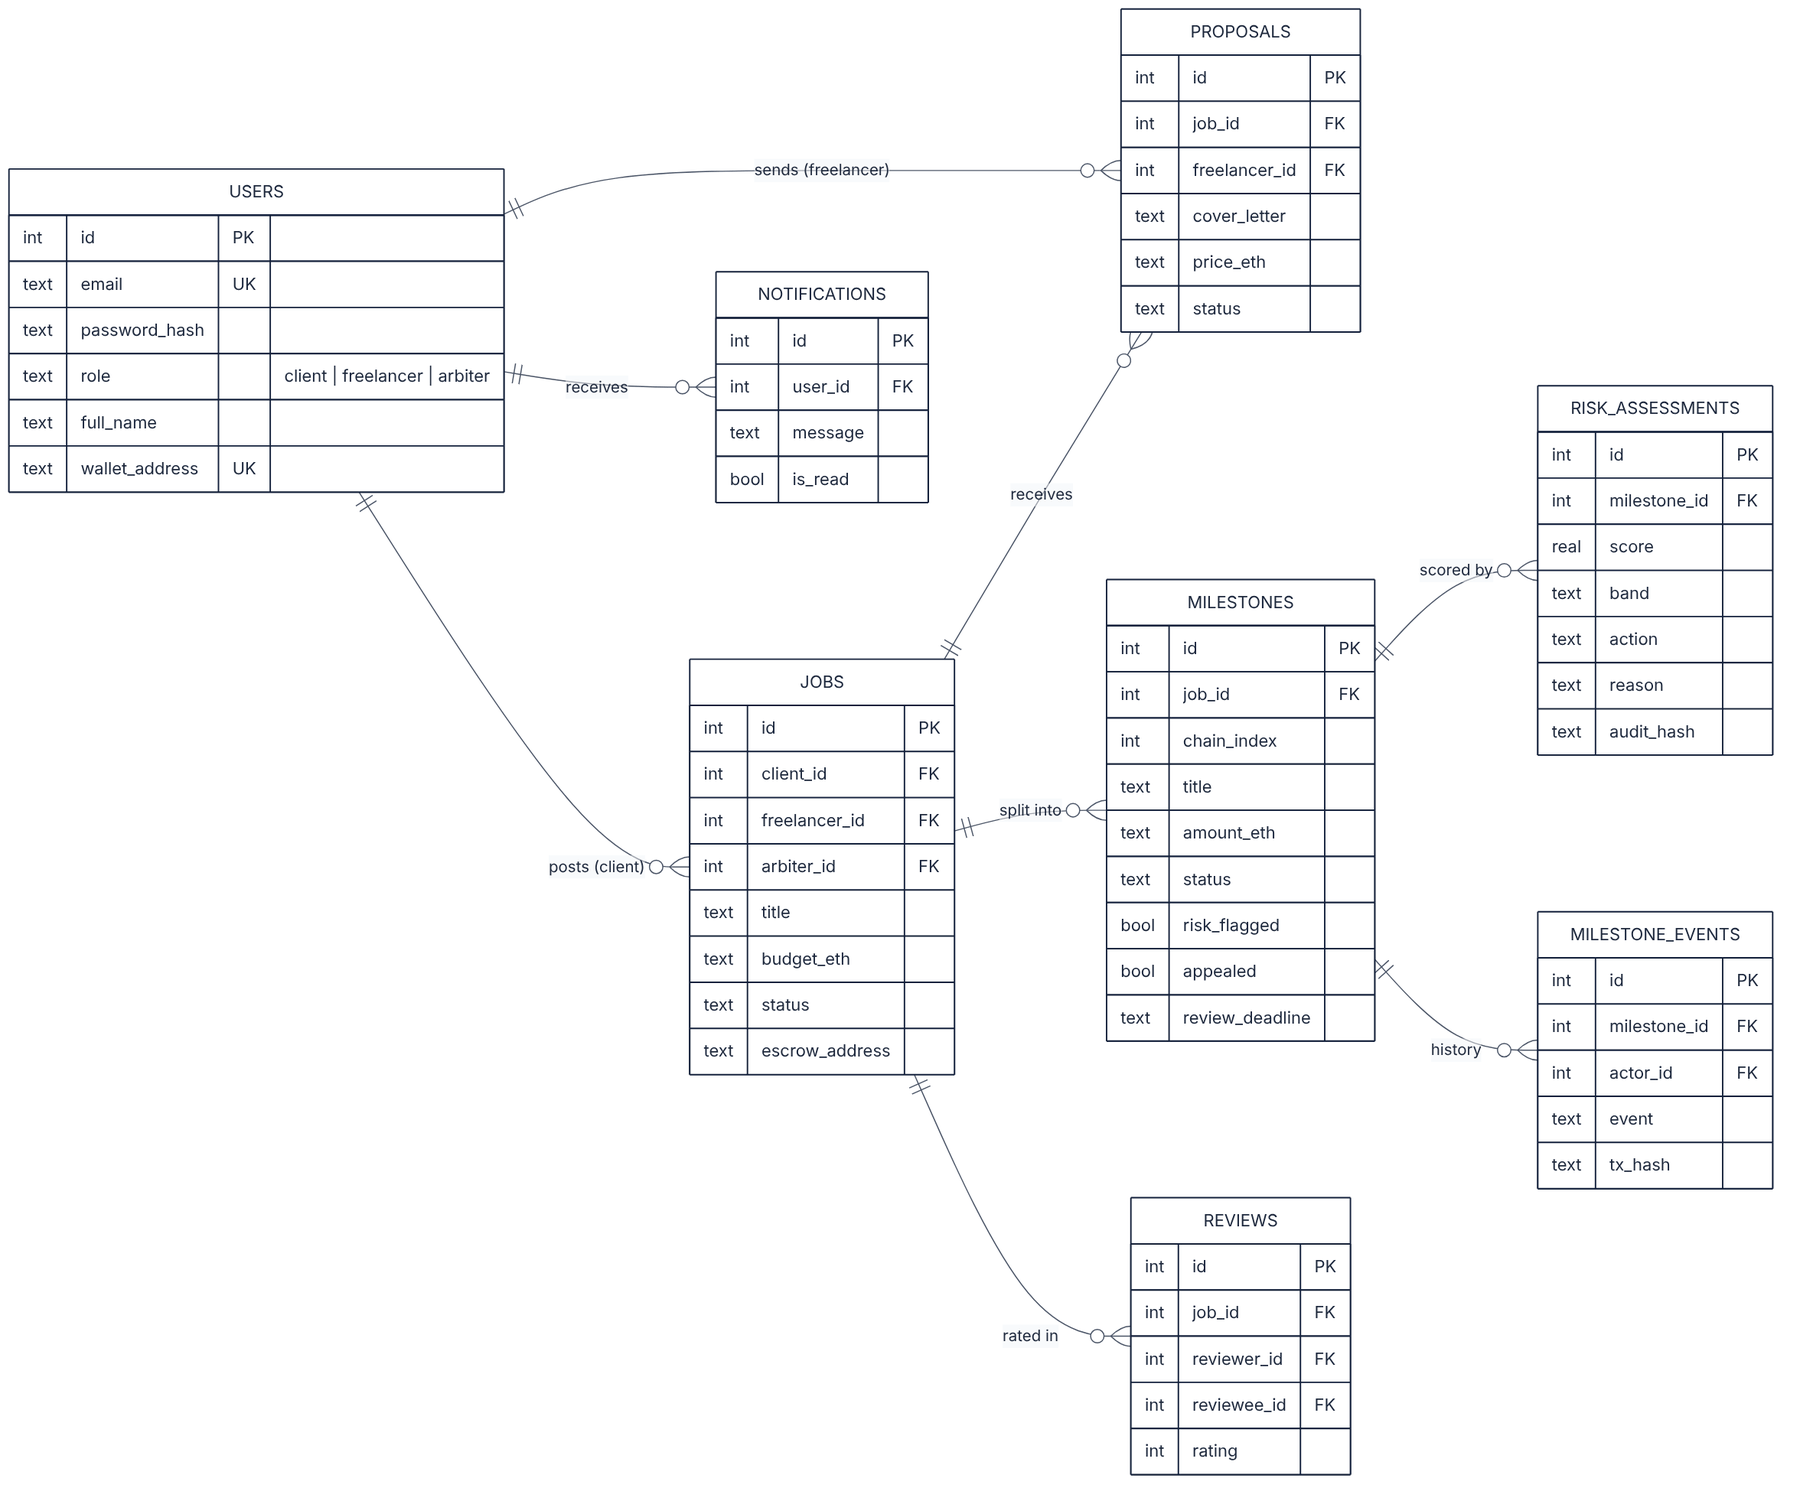
\includegraphics[width=\textwidth]{figures/er.png}
\caption{Entity-relationship diagram of the database.}
\label{fig:er}
\end{figure}

\section{Class diagram}
Figure~\ref{fig:class} shows how the modules depend on each other. The Express routers are the entry points and check roles. Two services wrap the outside systems: \texttt{ChainService} calls the contract through ethers.js and \texttt{RiskService} runs the Python engine through \texttt{predict\_cli.py}. The contract, risk engine, wallet model and audit log are the parts carried over from the proof of concept. The services are passed into the application when it starts, which lets the API tests use the real contract with a predictable stand-in for the risk engine.

\begin{figure}[htbp]
\centering
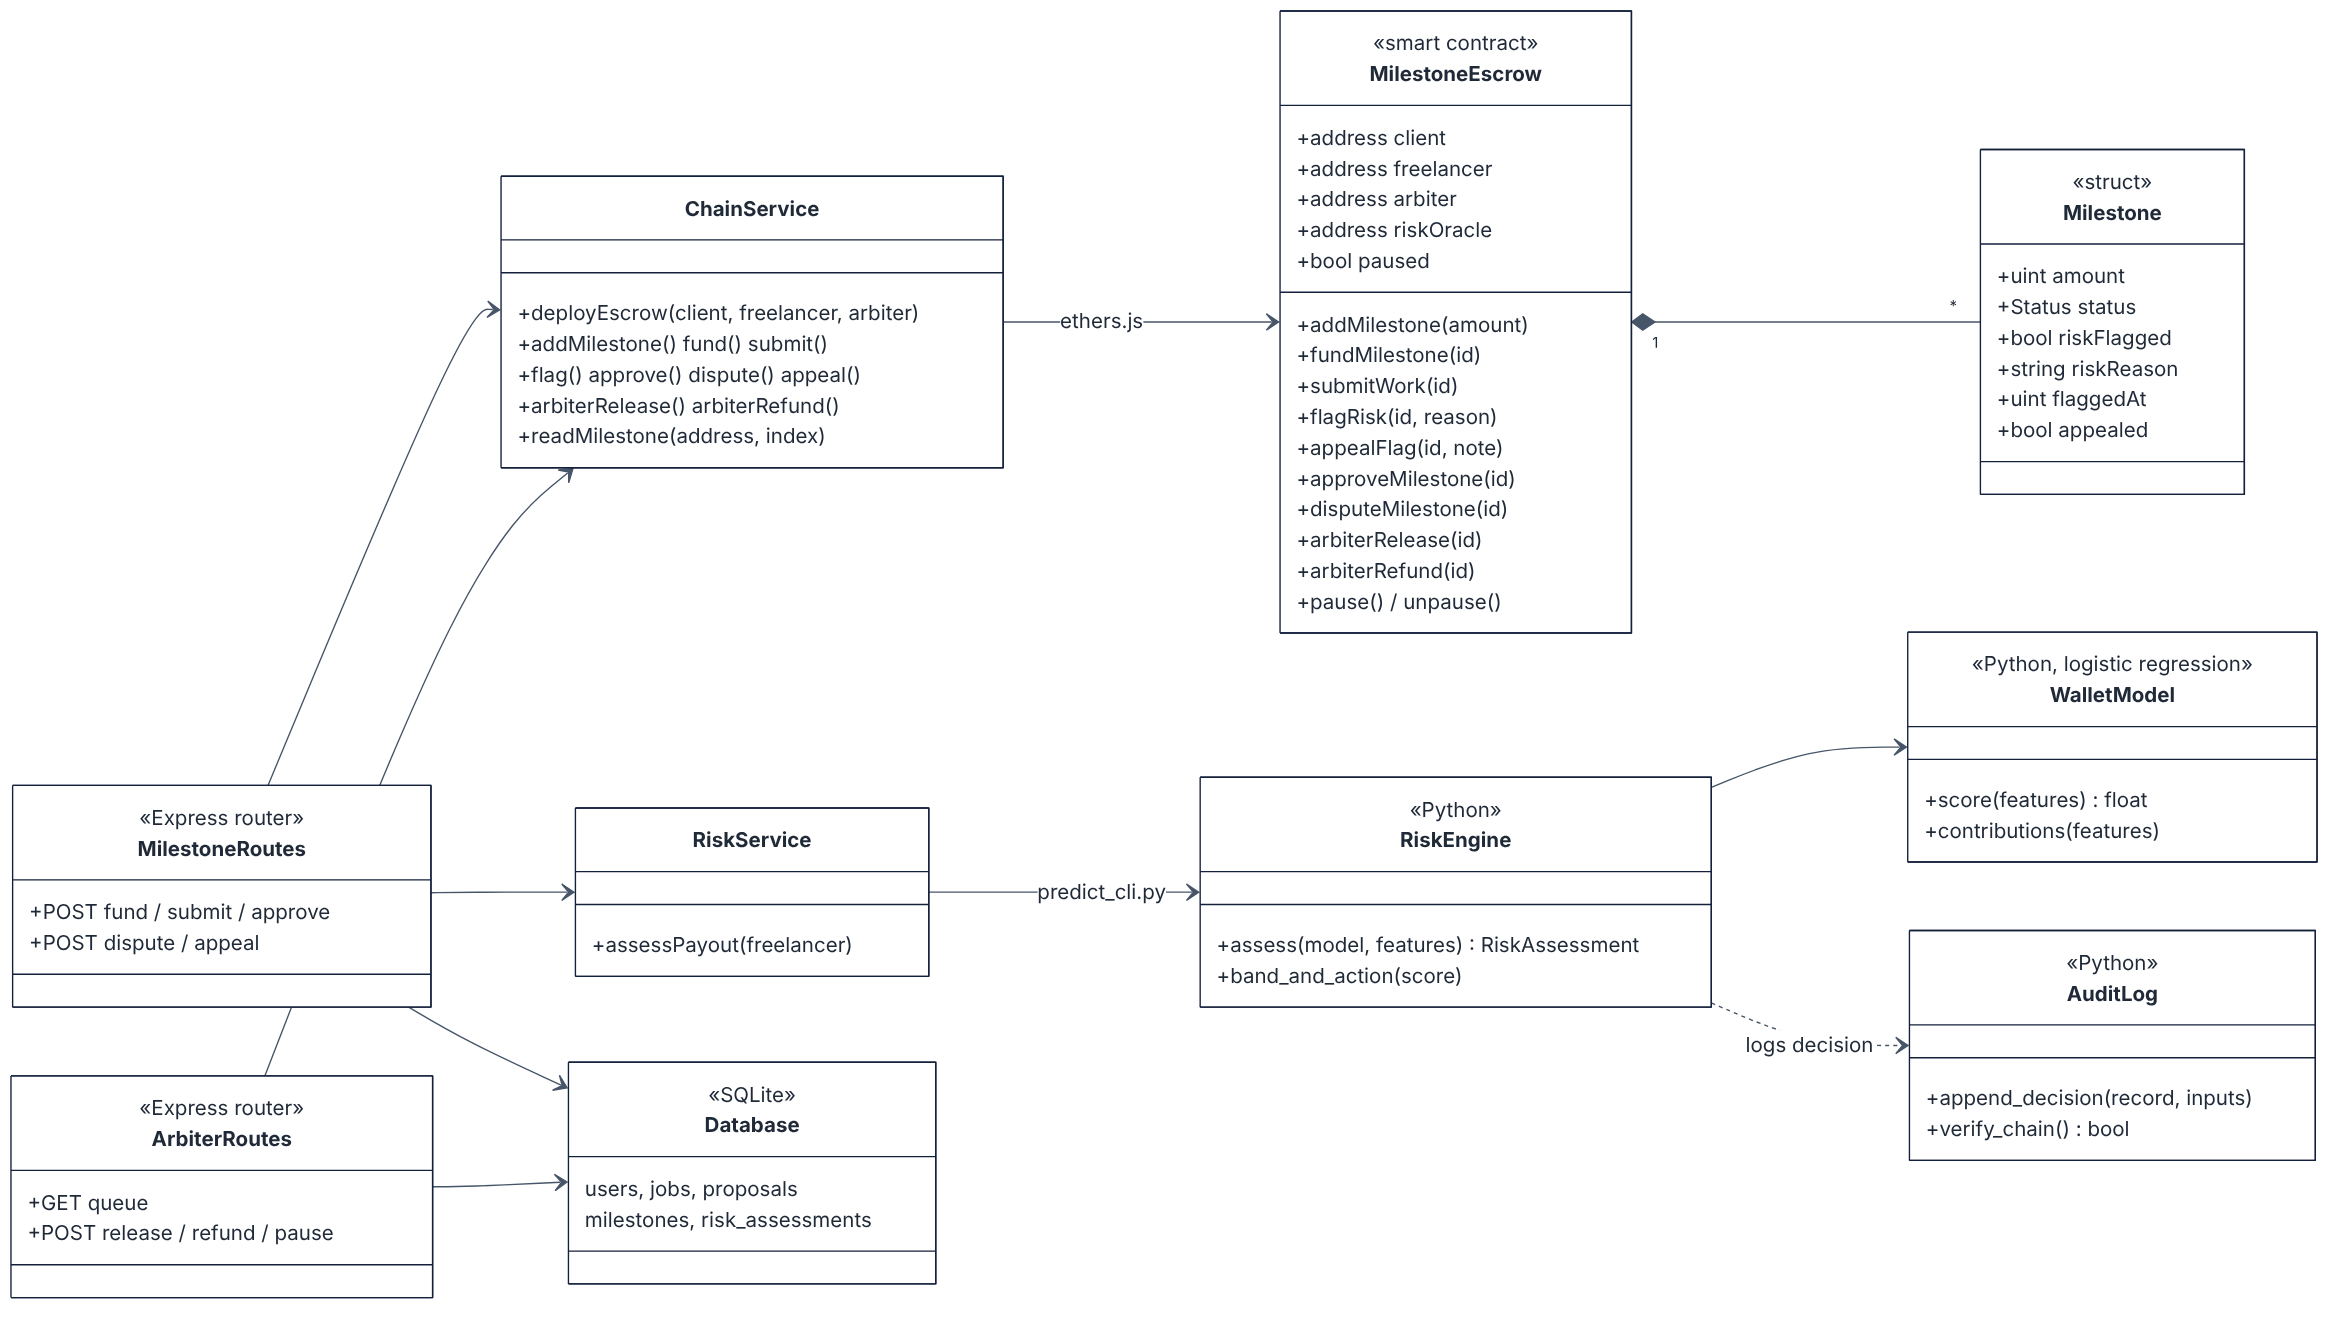
\includegraphics[width=\textwidth]{figures/class.png}
\caption{Class diagram of the main modules.}
\label{fig:class}
\end{figure}
